% ============================================================
%  Modul 3 — Perintah Dasar, Navigasi, dan Izin File Linux
% ============================================================

\chapter{Perintah Dasar, Navigasi, dan Izin File Linux}
\label{chap:modul-03}

% --- 1. Tujuan dan Output Praktikum ---
\section{Tujuan dan Output Praktikum}

\subsection{Tujuan Praktikum}
Setelah menyelesaikan praktikum ini, mahasiswa diharapkan mampu:
\begin{enumerate}
    \item Menjelaskan peran Sistem Operasi Linux beserta komponen intinya, seperti \textit{kernel} dan \textit{shell}.
    \item Menguraikan hierarki sistem berkas Linux dan melakukan navigasi direktori melalui Antarmuka Baris Perintah (CLI).
    \item Menerapkan aturan sintaks perintah Linux, termasuk penggunaan \textit{flag} dan argumen secara tepat.
    \item Mengoperasikan perintah-perintah dasar untuk manajemen berkas dan direktori (seperti \texttt{ls}, \texttt{cd}, \texttt{mkdir}, \texttt{rm}, \texttt{cp}, \texttt{mv}, \texttt{touch}, dan \texttt{cat}).
    \item Memahami konsep kepemilikan (\textit{ownership}) dan hak akses (\textit{permissions}) pada lingkungan berbasis Unix.
    \item Mengonfigurasi hak akses dan kepemilikan menggunakan \texttt{chmod} dan \texttt{chown}, serta memahami penggunaan otorisasi \textit{superuser} (\texttt{sudo}).
\end{enumerate}

\subsection{Output Praktikum}
Pada akhir praktikum ini, mahasiswa diharapkan menghasilkan luaran berupa:
\begin{itemize}
    \item Struktur direktori dan berkas rekayasa hasil manipulasi (pembuatan, penyalinan, pemindahan) yang dilakukan melalui terminal CLI.
    \item Dokumentasi log modifikasi hak akses berkas menggunakan kombinasi izin \textit{read, write,} dan \textit{execute}.
    \item Pemahaman perbedaan eksekusi perintah antara pengguna biasa (\texttt{\$}) dan \textit{superuser} (\texttt{\#}).
\end{itemize}

% --- 2. Dasar Teori ---
\newpage
\section{Dasar Teori}

\subsection{Komponen Utama Linux}
Linux adalah sistem operasi berbasis Unix yang bersifat \textit{open-source} \cite{das2012unix}. Untuk memahami cara kerjanya, pengguna perlu mengetahui tiga komponen utama berikut:
\begin{itemize}
    \item \textbf{\textit{Kernel}}: Bagian inti sistem operasi yang mengatur komunikasi antara perangkat keras (memori, prosesor) dan perangkat lunak \cite{Silberschatz2018}.
    \item \textbf{\textit{Terminal}}: Antarmuka berbasis teks tempat pengguna mengetikkan perintah \cite{shotts2019linux}.
    \item \textbf{\textit{Shell}}: Program penerjemah yang mengambil perintah dari terminal, mengeksekusinya, dan meneruskannya ke \textit{kernel}.
\end{itemize}

\subsection{Sistem Berkas dan Sintaks}
Sistem berkas pada Linux disusun dalam hierarki pohon terbalik dengan \textit{root} (\texttt{/}) sebagai induk tertingginya \cite{das2012unix}. Saat bernavigasi dan berinteraksi di Terminal, pengguna menggunakan sintaks dasar dengan struktur: \textbf{Perintah Dasar + \textit{Flag} + Argumen}.

\begin{itemize}
    \item \textbf{\textit{Flag}}: Opsi untuk mengubah perilaku perintah. Biasanya diawali tanda hubung "-" (contoh: \texttt{ls -l} untuk format detail).
    \item \textbf{Argumen}: Objek atau target data yang dikenai perintah, seperti nama file atau direktori (contoh: \texttt{rm dokumen.txt}) \cite{shotts2019linux}.
\end{itemize}

\subsection{Manajemen Hak Akses}

Setiap file dan direktori di Linux memiliki hak akses yang diatur untuk tiga kelompok pengguna: \textit{Owner} (Pemilik), \textit{Group} (Grup), dan \textit{Others} (Pengguna Lain). Terdapat tiga jenis izin utama:
\begin{itemize}
    \item \textbf{\textit{Read} (r)}: Hak untuk membaca atau melihat isi file/direktori.
    \item \textbf{\textit{Write} (w)}: Hak untuk mengubah, menambah, atau menghapus file.
    \item \textbf{\textit{Execute} (x)}: Hak untuk menjalankan file sebagai program (skrip).
\end{itemize}

Untuk mengubah izin ini, digunakan perintah \texttt{chmod}. Selain menggunakan huruf (\textit{r, w, x}), \texttt{chmod} juga sering digunakan dengan angka (mode oktal) seperti rincian berikut:

\begin{table}[H]
    \caption{Nilai Oktal Hak Akses File}
    \label{tab:chmod-oktal}
    \centering
    \begin{tabular}{|c|c|l|}
        \hline
        \textbf{Nilai} & \textbf{Simbol} & \textbf{Deskripsi} \\ \hline
        4 & \texttt{r--} & \textit{Read only} \\ \hline
        2 & \texttt{-w-} & \textit{Write only} \\ \hline
        1 & \texttt{--x} & \textit{Execute only} \\ \hline
        7 & \texttt{rwx} & Akses Penuh (4+2+1) \\ \hline
    \end{tabular}
\end{table}

Sementara itu, untuk mengubah pemilik dari sebuah file, sistem menggunakan perintah \texttt{chown}.

\vspace{0.5em}
\noindent\textbf{Membaca Output \texttt{ls -l}}

Perintah \texttt{ls -l} menampilkan detail lengkap setiap berkas. Contoh outputnya adalah:

\begin{lstlisting}[language=bash]
-rw-r--r-- 1 user group 1024 Jan  1 10:00 namaberkas.txt
\end{lstlisting}

Kolom pertama (\texttt{-rw-r--r--}) adalah \textit{permission string} 10 karakter yang dibaca dari kiri ke kanan:

\begin{table}[H]
    \caption{Breakdown \textit{Permission String} pada Output \texttt{ls -l}}
    \label{tab:ls-l-breakdown}
    \centering
    \begin{tabular}{|c|c|l|}
        \hline
        \textbf{Posisi} & \textbf{Contoh} & \textbf{Keterangan} \\ \hline
        1 & \texttt{-} & Tipe berkas: \texttt{-} = berkas biasa, \texttt{d} = direktori \\ \hline
        2--4 & \texttt{rw-} & Hak akses \textit{Owner}: \texttt{r}=baca, \texttt{w}=tulis, \texttt{-}=tanpa eksekusi \\ \hline
        5--7 & \texttt{r--} & Hak akses \textit{Group}: hanya baca \\ \hline
        8--10 & \texttt{r--} & Hak akses \textit{Others}: hanya baca \\ \hline
    \end{tabular}
\end{table}

Huruf yang tampil menandakan izin aktif, sedangkan tanda \texttt{-} berarti izin tersebut tidak diberikan. Sebagai contoh, \texttt{rwxr-x---} berarti: \textit{owner} memiliki akses penuh (\texttt{rwx}), \textit{group} hanya bisa baca dan eksekusi (\texttt{r-x}), sementara \textit{others} tidak memiliki hak akses sama sekali (\texttt{---}).

\subsection{Otorisasi \textit{Superuser}}
Beberapa perintah krusial yang dapat mengubah sistem secara fatal memerlukan hak administratif (\textit{superuser} atau \textit{root}). Anda dapat membedakan status Anda saat ini melalui tanda \textit{prompt} pada terminal:
\begin{itemize}
    \item Tanda dolar \textbf{\texttt{\$}}: Menandakan Anda bertindak sebagai \textit{user} biasa.
    \item Tanda pagar \textbf{\texttt{\#}}: Menandakan Anda bertindak sebagai \textit{root/superuser}.
\end{itemize}
Jika Anda login sebagai \textit{user} biasa namun perlu menjalankan perintah administratif, tambahkan perintah \textbf{\texttt{sudo}} (\textit{SuperUser DO}) di awal baris perintah \cite{shotts2019linux}.

\subsection{Perintah Dasar CLI}
Tabel \ref{tab:m03-dasar-teori} merangkum berbagai perintah esensial yang akan digunakan selama praktikum sesi ini.

\begin{table}[H]
    \caption{Tabel Ringkasan Perintah Dasar Linux}
    \label{tab:m03-dasar-teori}
    \centering
    \begin{tabular}{|l|p{10cm}|}
        \hline
        \textbf{Perintah} & \textbf{Deskripsi Singkat} \\ \hline
        \texttt{ls} & Melihat daftar file dan folder di dalam direktori. \\ \hline
        \texttt{ls -l} & Menampilkan daftar file beserta detail hak akses, pemilik, ukuran, dan tanggal modifikasi. \\ \hline
        \texttt{ls -la} & Sama seperti \texttt{ls -l}, tetapi juga menampilkan berkas tersembunyi (\textit{hidden files}) yang diawali titik (\texttt{.}). \\ \hline
        \texttt{pwd} & Memeriksa \textit{path} atau alamat direktori saat ini. \\ \hline
        \texttt{cd} & Berpindah ke direktori lain. \\ \hline
        \texttt{mkdir} & Membuat direktori (folder) baru. \\ \hline
        \texttt{rm} & Menghapus file atau direktori. \\ \hline
        \texttt{cp} & Menyalin file/direktori dari satu lokasi ke lokasi lain. \\ \hline
        \texttt{mv} & Memindahkan file atau mengubah nama file (\textit{rename}). \\ \hline
        \texttt{touch} & Membuat file teks kosong. \\ \hline
        \texttt{cat} & Menampilkan isi file teks langsung ke layar terminal. \\ \hline
        \texttt{nano} & Membuka teks editor bawaan terminal. \\ \hline
        \texttt{ps} & Menampilkan daftar proses yang sedang berjalan. \\ \hline
        \texttt{kill} & Menghentikan proses yang sedang berjalan. \\ \hline
        \texttt{chmod} & Mengubah hak akses (\textit{r, w, x}) sebuah file/direktori. \\ \hline
    \end{tabular}
\end{table}

% --- 3. Alat dan Bahan ---
\newpage
\section{Alat dan Bahan}
\label{sec:m03-alat-bahan}

\subsection{Perangkat Keras}
\begin{itemize}
	\item Laptop atau PC dengan prosesor minimal \textit{dual-core}.
	\item RAM minimal 4 GB (disarankan 8 GB untuk kinerja optimal).
	\item Ruang penyimpanan kosong minimal 25 GB.
\end{itemize}

\subsection{Perangkat Lunak}
\begin{itemize}
	\item Mesin Virtual Ubuntu (Guest OS) yang telah diinstal pada pertemuan sebelumnya.
\end{itemize}

% --- 4. Langkah-Langkah Praktikum ---
\newpage
\section{Langkah-Langkah Praktikum}

Berikut adalah tahapan-tahapan yang harus Anda selesaikan secara berurutan selama praktikum berlangsung:

\begin{enumerate}
    \item \textbf{Persiapan Lingkungan}
    
    Pastikan \textit{Virtual Machine} Ubuntu Anda sudah menyala dan Anda telah berhasil \textit{login}.
    \begin{enumerate}
        \item Buka terminal dengan menekan tombol \texttt{Ctrl+Alt+T} secara bersamaan.
        \item Gunakan perintah \texttt{pwd} untuk memeriksa \textit{path} atau alamat direktori yang saat ini diakses.
        \begin{lstlisting}[language=bash, caption={Perintah memverifikasi lokasi direktori saat ini}]
    $ pwd
        \end{lstlisting}
        Output yang dihasilkan adalah \textit{path} absolut direktori saat ini, misalnya:
        \begin{lstlisting}[language=bash]
    /home/namausername
        \end{lstlisting}
        \begin{figure}[H]
            \centering
            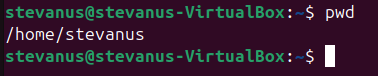
\includegraphics[width=0.75\textwidth]{Figure/03/gambar1.png}
            \caption{Tampilan terminal saat memverifikasi lokasi direktori menggunakan perintah \texttt{pwd}.}
            \label{fig:m03-gambar1}
        \end{figure}
    \end{enumerate}

    \vspace{1em}
    \item \textbf{Manipulasi Direktori dan Berkas}
    
    Pada tahap ini, Anda akan membuat, menyalin, dan memindahkan berkas menggunakan perintah dasar CLI.
    \begin{enumerate}
        \item Buatlah sebuah direktori baru bernama \texttt{data} dan masuk ke dalamnya menggunakan perintah \texttt{cd}.
        \begin{lstlisting}[language=bash, caption={Membuat dan masuk ke direktori baru}]
    $ mkdir data
    $ cd data
        \end{lstlisting}
        \begin{figure}[H]
            \centering
            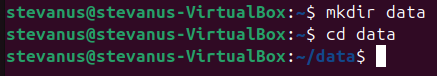
\includegraphics[width=0.75\textwidth]{Figure/03/gambar2.png}
            \caption{Proses pembuatan direktori baru dan berpindah ke dalamnya.}
            \label{fig:m03-gambar2}
        \end{figure}
        
        \item Buatlah berkas teks baru menggunakan teks editor \texttt{nano}.
        \begin{lstlisting}[language=bash, caption={Membuka editor nano}]
    $ nano belajarlinux.txt
        \end{lstlisting}
        Ketikkan Nama dan NIM Anda di dalamnya. Simpan perubahan dengan menekan \texttt{Ctrl+O} lalu tekan \texttt{Enter}. Setelah itu, keluar dari editor dengan menekan \texttt{Ctrl+X}.
        \begin{figure}[H]
            \centering
            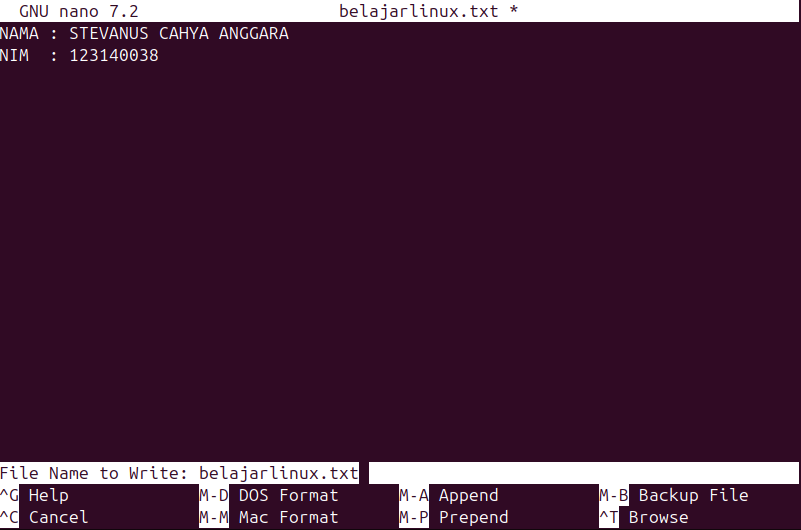
\includegraphics[width=0.75\textwidth]{Figure/03/gambar4.png}
            \caption{Tampilan editor teks \texttt{nano} saat mengedit berkas.}
            \label{fig:m03-gambar3}
        \end{figure}
        
        \item Tampilkan isi berkas yang baru saja dibuat ke layar terminal menggunakan perintah \texttt{cat}.
        \begin{lstlisting}[language=bash, caption={Menampilkan isi berkas}]
    $ cat belajarlinux.txt
        \end{lstlisting}
        Isi berkas akan langsung tercetak di terminal. Contoh output sesuai data yang Anda masukkan:
        \begin{lstlisting}[language=bash]
    Nama: Budi Santoso
    NIM: 12345678
        \end{lstlisting}

        \item Buat direktori baru bernama \texttt{data2} dan salin berkas \texttt{belajarlinux.txt} ke dalamnya.
        \begin{lstlisting}[language=bash, caption={Menyalin berkas menggunakan cp}]
    $ mkdir data2
    $ cp belajarlinux.txt data2/
    $ ls data2/
        \end{lstlisting}
        \begin{figure}[H]
            \centering
            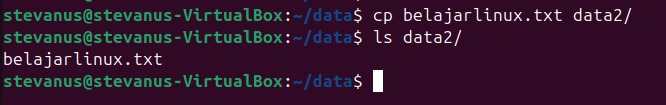
\includegraphics[width=0.75\textwidth]{Figure/03/gambar5.png}
            \caption{Proses penyalinan berkas ke dalam direktori tujuan beserta verifikasinya.}
            \label{fig:m03-gambar5}
        \end{figure}
        
        \item Pindah ke direktori \texttt{data2} dan ubah nama berkas menggunakan perintah \texttt{mv}.
        \begin{lstlisting}[language=bash, caption={Mengubah nama berkas menggunakan mv}]
    $ cd data2
    $ mv belajarlinux.txt belajarlagi.txt
    $ ls
        \end{lstlisting}
        \begin{figure}[H]
            \centering
            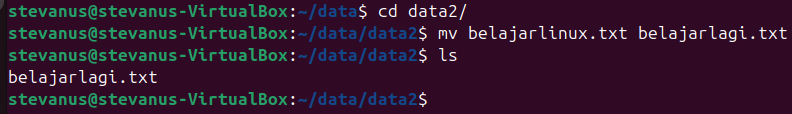
\includegraphics[width=0.75\textwidth]{Figure/03/gambar6.png}
            \caption{Pengubahan nama berkas menggunakan perintah \texttt{mv}.}
            \label{fig:m03-gambar6}
        \end{figure}
    \end{enumerate}

    \vspace{1em}
    \item \textbf{Manipulasi Hak Akses}
    
    Pada tahap ini, Anda akan mencoba mengubah "kunci gembok" (\textit{permissions}) dari berkas yang sudah dibuat sebelumnya. 
    \begin{enumerate}
        \item Hapus hak akses baca (\textit{read}) dan tulis (\textit{write}) untuk pengguna asing (\textit{others}) pada berkas \texttt{belajarlagi.txt} dengan menggunakan parameter \texttt{o-rw}.
        \begin{lstlisting}[language=bash, caption={Mengubah hak akses berkas (symbolic mode)}]
    $ chmod o-rw belajarlagi.txt

    # Verifikasi perubahan hak akses, perhatikan deretan huruf di sebelah kiri
    $ ls -l
        \end{lstlisting}

        \noindent\textbf{Catatan — Mode Numerik (Oktal):} Perintah di atas menggunakan \textit{symbolic mode}. Perintah yang sama dapat ditulis dengan \textit{numeric mode} menggunakan angka oktal dari tabel \ref{tab:chmod-oktal}. Sebagai contoh, \texttt{chmod 640 belajarlagi.txt} memberikan efek yang setara:
        \begin{itemize}
            \item \textbf{6} (4+2) $\rightarrow$ \textit{Owner}: baca dan tulis (\texttt{rw-})
            \item \textbf{4} $\rightarrow$ \textit{Group}: hanya baca (\texttt{r--})
            \item \textbf{0} $\rightarrow$ \textit{Others}: tanpa akses (\texttt{---})
        \end{itemize}
        \begin{lstlisting}[language=bash, caption={Perintah yang setara menggunakan numeric mode}]
    $ chmod 640 belajarlagi.txt
        \end{lstlisting}
        \begin{figure}[H]
            \centering
            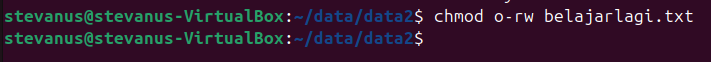
\includegraphics[width=0.75\textwidth]{Figure/03/gambar7.png}
            \caption{Status hak akses berkas sebelum dilakukan modifikasi.}
            \label{fig:m03-gambar7}
        \end{figure}
        \begin{figure}[H]
            \centering
            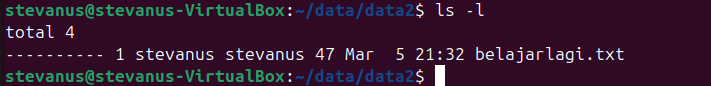
\includegraphics[width=0.75\textwidth]{Figure/03/gambar8.png}
            \caption{Status hak akses berkas setelah modifikasi dengan \texttt{chmod}.}
            \label{fig:m03-gambar8}
        \end{figure}
        
        \item Coba ubah kepemilikan berkas tersebut menjadi milik pengguna \texttt{root}.

        Operasi \texttt{chown} (change owner) mengubah siapa yang tercatat sebagai \textit{owner} dari sebuah berkas. Karena mengubah kepemilikan merupakan tindakan administratif yang berdampak pada keamanan sistem, perintah ini \textbf{memerlukan hak} \textit{superuser} dan harus dijalankan dengan \texttt{sudo}.
        \begin{lstlisting}[language=bash, caption={Menggunakan sudo untuk mengubah owner ke root}]
    $ sudo chown root belajarlagi.txt
    $ ls -l
        \end{lstlisting}
        Setelah perintah ini, kolom kepemilikan pada output \texttt{ls -l} akan berubah dari nama pengguna Anda menjadi \texttt{root}. Akibatnya, Anda \textbf{tidak lagi dapat mengedit} berkas tersebut tanpa menggunakan \texttt{sudo}, karena \textit{owner}-nya kini bukan Anda.

        Untuk mengembalikan kepemilikan ke pengguna Anda sendiri, jalankan:
        \begin{lstlisting}[language=bash, caption={Mengembalikan kepemilikan berkas ke pengguna semula}]
    $ sudo chown $USER belajarlagi.txt
        \end{lstlisting}
        Variabel \texttt{\$USER} secara otomatis merujuk ke nama pengguna yang sedang aktif.
        \begin{figure}[H]
            \centering
            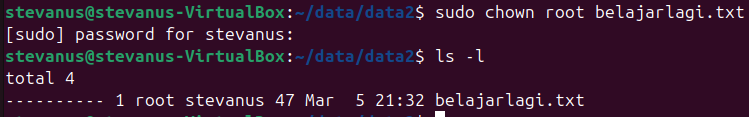
\includegraphics[width=0.75\textwidth]{Figure/03/gambar9.png}
            \caption{Perubahan kepemilikan berkas menjadi pengguna \texttt{root}.}
            \label{fig:m03-gambar9}
        \end{figure}
    \end{enumerate}

\end{enumerate}

% --- 5. Penanganan Kesalahan Umum ---
\newpage
\section{Penanganan Kesalahan Umum}
\label{sec:m03-troubleshooting}

Berikut adalah pesan kesalahan yang sering dijumpai selama praktikum beserta cara mengatasinya:

\begin{table}[H]
    \caption{Kesalahan Umum dan Cara Mengatasinya}
    \label{tab:m03-troubleshooting}
    \centering
    \begin{tabular}{|p{5.5cm}|p{4cm}|p{4.5cm}|}
        \hline
        \textbf{Pesan Kesalahan} & \textbf{Penyebab Umum} & \textbf{Cara Mengatasi} \\ \hline
        \texttt{Permission denied} & Anda tidak memiliki hak akses untuk membaca, menulis, atau menjalankan berkas tersebut. & Periksa permission dengan \texttt{ls -l}. Gunakan \texttt{chmod} untuk menyesuaikan, atau tambahkan \texttt{sudo} jika aksi memerlukan hak administratif. \\ \hline
        \texttt{mkdir: cannot create directory 'data': File exists} & Direktori dengan nama yang sama sudah ada. & Gunakan nama direktori lain, atau hapus direktori lama terlebih dahulu dengan \texttt{rm -r namadir}. \\ \hline
        \texttt{No such file or directory} & Berkas atau direktori yang dituju tidak ditemukan di \textit{path} yang diberikan. & Pastikan ejaan nama berkas benar. Gunakan \texttt{ls} untuk melihat isi direktori saat ini, dan \texttt{pwd} untuk mengecek lokasi Anda. \\ \hline
        \texttt{sudo: command not found} & Perintah \texttt{sudo} tidak tersedia (jarang terjadi di Ubuntu). & Pastikan Anda menggunakan distribusi Ubuntu yang sudah dikonfigurasi. Hubungi asisten praktikum jika masalah berlanjut. \\ \hline
        \texttt{bash: nano: command not found} & Editor \texttt{nano} belum terpasang. & Pasang dengan perintah \texttt{sudo apt install nano}. \\ \hline
    \end{tabular}
\end{table}